\documentclass[12pt,letterpaper]{article}

% ============================================================
% Packages
% ============================================================
\usepackage[margin=1in,headheight=15pt]{geometry}
\usepackage{fontspec}
\setmainfont{TeX Gyre Heros}
\setmonofont{Latin Modern Mono}
\usepackage{setspace}
\usepackage{titlesec}
\usepackage{enumitem}
\usepackage{listings}
\usepackage{amsmath}
\usepackage{amssymb}
\usepackage{parskip}
\usepackage{hyperref}
\usepackage{cleveref}
\usepackage{fancyhdr}
\usepackage{lastpage}
\usepackage[numbers,sort&compress]{natbib}
\usepackage{graphicx}

\raggedright
\hyphenpenalty=10000
\exhyphenpenalty=10000

% ============================================================
% Page style
% ============================================================
\pagestyle{fancy}
\fancyhf{}
\chead{Provisional Patent Application --- Spiker}
\rfoot{Page \thepage\ of \pageref{LastPage}}
\renewcommand{\headrulewidth}{0.4pt}

% ============================================================
% Section formatting
% ============================================================
\titleformat{\section}{\normalfont\large\bfseries\uppercase}{}{0em}{}[\titlerule]
\titleformat{\subsection}{\normalfont\normalsize\bfseries}{}{0em}{}
\titleformat{\subsubsection}{\normalfont\normalsize\itshape}{}{0em}{}

% ============================================================
% Listings (code blocks)
% ============================================================
\lstset{
  basicstyle=\ttfamily\small,
  frame=single,
  breaklines=true,
  columns=fullflexible,
  keepspaces=true
}

% ============================================================
% Claim counter and formatting
% ============================================================
\newcounter{claimnum}
\setcounter{claimnum}{0}

\newenvironment{claim}[1][]{%
  \refstepcounter{claimnum}%
  \noindent\textbf{Claim \theclaimnum.}\space
}{%
  \par\medskip
}

% ============================================================
% Reference labels
% ============================================================
% All bibliography entries use \bibitem with numeric keys.
% See References section at end.

% ============================================================
\begin{document}
% ============================================================

% ============================================================
% Title block
% ============================================================
\begin{center}
  {\LARGE\bfseries Provisional Patent Application}\\[1.5em]
  {\large\bfseries Hardware Memory Protection System Using Base--Limit Register Pairs with Cryptographically Indistinguishable Invalid Access Responses}\\[1.5em]
  \textbf{Inventor:} Nick Spiker\\
  \textbf{Filing Date:} [March 14, 2026]\\
  \textbf{Prior Art Established:} January 1, 2025 (ferros architecture document)
\end{center}

\vspace{1em}
\hrule
\vspace{2em}

% ============================================================
\section{Abstract}
% ============================================================

A memory protection architecture for general-purpose operating systems
providing process isolation thru per-process hardware base and limit
registers without page tables or virtual memory translation, combined with
a mechanism wherein invalid memory accesses return computationally
indistinguishable responses derived from a hardware-protected secret key
and the accessed address, preventing information disclosure about valid
memory region boundaries by any sequence of memory access attempts.

The hardware key register output is physically wired to exactly one
destination: the $f$ computation logic. No path from the key register
to any data bus exists in the circuit netlist. This is a structural
property of the hardware, not a software-enforced policy. An attacker
probing the key register's address receives cipher output per the
invalid access response mechanism --- a consequence of the address
falling outside valid process bounds, independent of the key register's
own wiring. The two protections are structurally independent and
mutually reinforcing.

In a further embodiment, physical RAM is encrypted thruout using a
stream cipher keyed by a hardware-protected key.
This produces data and computational indistinguishability across three
distributions: raw physical RAM reads, valid software memory reads,
and invalid software memory reads are all computationally
indistinguishable without knowledge of the hardware-protected keys.
An attacker with complete software and physical access to bus signal
values obtains no information about memory contents, valid address
regions, or process memory boundaries.

In a further embodiment, both the valid memory data path and the
$f$-derived response path execute unconditionally on every memory
access, with a final multiplexer selecting the output. This extends
indistinguishability to the physical side channel domain: power
consumption and switching activity are identical for valid and invalid
accesses, defeating power analysis attacks.

The address space is toroidal under two's complement arithmetic: no
address is structurally privileged, wraparound is handled correctly
without special-case logic, and the null pointer dereference
vulnerability class does not exist in this architecture.

% ============================================================
\section{Field of the Invention}
% ============================================================

Memory protection hardware and operating system architecture providing
process isolation thru arithmetic bounds checking as a complete
replacement for virtual memory and page table systems, combined with
a cryptographically indistinguishable response mechanism for invalid
memory accesses.

% ============================================================
\section{Background}
% ============================================================

\subsection{The Problem With Page Tables}

All known general-purpose operating systems use virtual memory and
page tables for process memory isolation. This approach requires:

\begin{itemize}[noitemsep]
  \item A Memory Management Unit (MMU) performing virtual-to-physical
        address translation on every memory access
  \item Translation Lookaside Buffer (TLB) hardware caching recent translations
  \item Page tables stored in RAM, requiring additional memory accesses on TLB miss
  \item Page-aligned allocations (typically 4\,KB, 2\,MB, or 1\,GB granularity)
  \item Complex kernel code for page table management
\end{itemize}

This architecture has well-documented problems:

\textbf{Performance.}
TLB miss incurs 4--5 memory reads ($\sim$100--500 cycles).
TLB hit requires 3--5 cycles minimum.
Latency is non-deterministic, varying with working set size and TLB pressure.

\textbf{Page granularity waste and unintended valid memory.}
Page table systems allocate memory in fixed-size pages (typically 4\,KB).
A process requesting a single byte receives a full 4\,KB page:
4,095 bytes of valid, addressable memory the process did not request
and may not have initialized.
A process requesting 800\,MB receives memory rounded up to the nearest
page boundary.
This over-allocation has two consequences.
First, the bytes between the requested size and the page boundary are
valid memory belonging to the process --- adjacent allocations on the
same page may read uninitialized data from neighboring allocations,
a well-documented source of information disclosure vulnerabilities.
Second, describing an 800\,MB allocation requires approximately 204,800
page table entries (800\,MB $\div$ 4\,KB), each consuming 8 bytes of
kernel RAM, totaling $\sim$1.6\,MB of overhead just to describe one
process's allocation.
A system running many processes with large working sets carries
correspondingly large page table structures consuming physical RAM
and generating TLB pressure.

\textbf{Alignment constraints.}
Page tables require base addresses aligned to page size.
MMIO registers at arbitrary physical addresses require mapping entire pages,
potentially granting access to adjacent hardware registers belonging to different
security domains.

\textbf{Complexity.}
The Linux kernel contains millions of lines of page table management code,
including demand paging, swap, huge pages, NUMA, OOM killer, and related
subsystems --- each a source of security vulnerabilities.

\textbf{Information disclosure via deterministic fault responses.}
On all current operating systems, accessing memory outside a process's
valid region produces a deterministic, observable signal: a page fault,
SIGSEGV, bus error, or equivalent.
This signal is itself information: the attacker learns that the probed
address was outside valid memory.
By systematically probing addresses and observing which produce faults
and which succeed, an attacker can enumerate valid memory region
boundaries.
On x86-64, this binary search converges to 4\,KB granularity ---
the page size --- in $O(\log N)$ probes, where $N$ is the address
space size.
With 2\,MB huge pages the granularity is coarser but the attack
remains practical.
Address Space Layout Randomization (ASLR) raises the cost of this
search but does not eliminate it: once a single fault-vs-success
pair is observed, the search proceeds normally.
Timing side channels~\cite{hund_timing} further reduce the cost
of ASLR bypass.
This invention eliminates the information disclosure problem at its
root: invalid accesses produce cipher output indistinguishable from
valid data, providing no signal that an invalid address was probed.

\subsection{Prior Art and Its Limitations}

\textbf{Base and limit registers (1960s--1970s mainframes).}
Used in early systems including Cray supercomputers for memory partitioning.
Required contiguous physical memory allocation.
Replaced by virtual memory due to external fragmentation.
No cryptographic response mechanism.
Not used in modern general-purpose operating systems~\cite{silberschatz}.

\textbf{CHERI (Capability Hardware Enhanced RISC Instructions).}
University of Cambridge / SRI International, active development since 2010.
Embeds base and bounds metadata in capability fat pointers (128-bit or 256-bit).
Operates \emph{alongside} conventional MMU and page tables as a hybrid model ---
explicitly not a replacement for virtual memory.
Invalid capability access produces a hardware exception.
Does not return cryptographically random or cipher-based data on invalid access.
Requires page tables to remain operational~\cite{cheri_isca,cheri_isa}.

\textbf{Mill Computing architecture.}
Protection Lookaside Buffer (PLB) separate from address translation,
operating on virtual addresses.
Still uses virtual memory and address translation.
Invalid memory access produces NaR (Not a Result) metadata tag ---
a special sentinel value, not cryptographically random data.
Does not make invalid access indistinguishable from valid access~\cite{mill}.

\textbf{Intel MPX (Memory Protection Extensions).}
Bounds registers supplementing existing page-table-based protection.
Deprecated in 2019.
Invalid access produces \texttt{\#BR} exception ---
not cryptographically random data~\cite{mpx}.

\textbf{ARM MTE (Memory Tagging Extension).}
Tag bits on memory allocations for temporal and spatial safety.
Still requires MMU and page tables.
Invalid tag access produces exception ---
not random data~\cite{arm_mte}.

\textbf{ASLR (Address Space Layout Randomization).}
Randomizes base addresses of memory regions to make probing harder.
Still uses page tables.
Defeated by information leaks (Spectre, Meltdown, side channels).
Provides probabilistic obscurity, not cryptographic guarantees~\cite{pax_aslr,hund_timing}.

% ============================================================
\section{Summary of the Invention}
% ============================================================

The invention provides a memory protection architecture comprising:

\begin{enumerate}[noitemsep]
  \item Per-process hardware base and limit register pairs replacing page tables
        as the sole memory isolation mechanism, with physical address equal to
        virtual address (MMU disabled or bypassed)

  \item A two-operation bounds validation --- subtract base, compare to limit ---
        of deterministic, constant latency

  \item For invalid accesses: a response derived from a hardware-protected secret
        key and the accessed address, such that the response is computationally
        indistinguishable from valid memory data without knowledge of the secret key

  \item A hardware key register whose read-disable property is enforced by the same
        mechanism as invalid access response (Claim~2): any instruction that would
        read the register falls outside any valid process bounds and therefore
        receives the same cipher-derived output as any other invalid access,
        with no separate read path existing in hardware

  \item A process table maintained by the kernel associating each running process
        with its base and limit registers; all address inputs to the response
        function are in the context of a process table entry and are natively
        hardware-word-width (usize), requiring no extension or truncation
\end{enumerate}

\textbf{Self-referential key protection.}
The hardware secret key is protected by the same mechanism it participates in.
An attacker attempting to read the key register receives cipher-derived output
indistinguishable from any other invalid access.
The protection is uniform: there is no privileged path to key material at any
software level, including kernel privilege.
This property is intrinsic to the hardware wiring, not a software-enforced policy.

% ============================================================
\section{Detailed Description}
% ============================================================

\subsection*{Independent Claim 1: Base--Limit Register Memory Protection
  (No Page Tables)}

A memory protection system comprising:

\begin{enumerate}[label=(\alph*),noitemsep]
  \item At least one base register per process storing a physical base address
  \item At least one limit register per process storing a maximum accessible
        offset from the base address
  \item Hardware logic performing on every memory access:
        \begin{lstlisting}
offset = accessed_address - base_register
valid  = (offset < limit_register)   // unsigned comparison
        \end{lstlisting}
  \item No page table data structure required for process memory isolation
  \item No TLB required for process memory isolation
  \item Arbitrary base address alignment: base register may contain any address,
        not constrained to page boundaries
  \item Arbitrary allocation size: limit register may specify any byte count,
        not constrained to power-of-two page sizes
  \item Physical addresses equal virtual addresses; the MMU is disabled or
        bypassed entirely, eliminating address translation overhead
  \item A kernel-maintained process table associating each running process with
        one or more base--limit register pairs; physical memory assignment is
        managed directly by the kernel without page table data structures
\end{enumerate}

\textbf{Distinction from prior art.}
Classic base/limit systems~\cite{silberschatz} required page-aligned contiguous
physical memory and were abandoned due to fragmentation.
This invention operates in a modern general-purpose OS context with no page tables,
no MMU translation, and no alignment constraints.
CHERI~\cite{cheri_isca} uses similar bounds checking but retains page tables and
MMU as required components and does not disable virtual memory.

\medskip

\subsection*{Independent Claim 2: Cryptographically Indistinguishable
  Invalid Access Response}

A memory protection system wherein invalid memory accesses return data computed as:
\[
  \textit{response} = f(\textit{secret\_key},\; \textit{accessed\_address})
\]
where:
\begin{enumerate}[label=(\alph*),noitemsep]
  \item \textit{secret\_key} is stored in a hardware register enforced
        read-disabled as described in Claim~4
  \item \textit{accessed\_address} is a hardware-word-width (usize) value
        drawn from the process table context; no extension or truncation of the
        address is required
  \item $f$ is a deterministic function such that:
    \begin{itemize}[noitemsep]
      \item The same address always produces the same response for a given key
      \item The response is computationally indistinguishable from valid memory
            contents without knowledge of \textit{secret\_key}
      \item The response is computed in hardware
    \end{itemize}
  \item No error signal, exception, fault, or otherwise distinguishable response
        is generated for invalid accesses
\end{enumerate}

\textbf{Distinction from prior art:}
\begin{itemize}[noitemsep]
  \item Page fault / SIGSEGV (all conventional OS): deterministic error,
        reveals boundary location
  \item NaR (Mill Computing~\cite{mill}): special sentinel value,
        distinguishable from valid data by inspecting metadata
  \item Hardware exception (CHERI~\cite{cheri_isca}, MPX~\cite{mpx},
        MTE~\cite{arm_mte}): deterministic error signal
  \item Zero / fixed value: distinguishable from valid data by inspection
  \item Bus error / hang: distinguishable by timing
\end{itemize}

This invention is the first to provide computationally indistinguishable responses
for invalid memory accesses.

\medskip

\subsection*{Dependent Claim 3: Double-Read Attack Resistance
  (depends on Claim~2)}

A memory protection system according to Claim~2 wherein the deterministic
property of $f$ prevents double-read distinguisher attacks:

\begin{enumerate}[label=(\alph*),noitemsep]
  \item An attacker reading an invalid address twice receives identical values
  \item Valid memory and invalid memory are indistinguishable by repeated
        access patterns
  \item Achieved by: $f(\textit{secret\_key}, \textit{address})$ being
        deterministic for a given (key, address) pair while being computationally
        random without knowledge of \textit{secret\_key}
\end{enumerate}

\medskip

\subsection*{Dependent Claim 4: Hardware Key Protection
  (depends on Claim~2)}

A memory protection system according to Claim~2 wherein:

\begin{enumerate}[label=(\alph*),noitemsep]
  \item \textit{secret\_key} is stored in a hardware register whose
        output is physically wired to exactly one destination: the
        input of the $f$ computation logic (the ARX compression
        function, block cipher, or equivalent per Claim~7).
        No other wire, bus connection, or signal path from the
        key register output exists in the hardware implementation.
        This is a property of the circuit netlist, not of software
        policy or privilege gating.

  \item Specifically: the key register output is not connected to the
        processor data bus, not connected to any multiplexer whose
        other input reaches the data bus, and not readable by any
        instruction in the ISA. The absence of a read path is
        structural --- there is no gate to bypass, no privilege check
        to circumvent, no microcode path to exploit. The key material
        cannot appear on the data bus because no wire connecting the
        key register to the data bus exists.

  \item The read-disable property is therefore not circular with
        respect to Claim~2. Claim~2 describes the response produced
        when a software access falls outside valid bounds. Claim~4
        describes a separate physical constraint: the key register
        output wire terminates at the $f$ logic and nowhere else.
        An attacker probing the key register's address receives
        $f(\textit{secret\_key}, \textit{address})$ per Claim~2
        because that address is outside any valid process region ---
        not because the key register has a special protection
        mechanism. The two properties are independent and
        mutually reinforcing, not circularly dependent.

  \item The register accepts writes (to install a new key via a
        privileged instruction) but the write path is one-way into
        the register storage element only; the output of the storage
        element is wired exclusively to the $f$ logic as described
        in (a).

  \item The key is derived fresh at each boot:
        \[
          \textit{key} = \textit{cipher}(\textit{device\_key},\; \textit{boot\_nonce})
        \]
        where \textit{device\_key} is a per-device secret stored in
        one-time-programmable (OTP) fuses or equivalent non-volatile
        hardware storage, similarly having no software-readable output path.

  \item Key erasure: power removal causes immediate loss of
        \textit{secret\_key} (volatile register storage).
        \textit{device\_key} persists in OTP but is not sufficient
        to reconstruct \textit{secret\_key} without the
        \textit{boot\_nonce} consumed at boot time.
\end{enumerate}

\textbf{Result.}
An attacker with full software access including kernel privilege cannot extract
\textit{secret\_key} because no instruction causes the processor to place
the register contents on any data bus --- there is no such path in the
circuit.
An attacker probing the key register's memory address receives cipher output
per Claim~2 because that address is outside all valid process regions.
The two protections are structurally independent; neither depends on the
other for its validity.

\medskip

\subsection*{Dependent Claim 5: MMIO Grant Arbitrary Granularity
  (depends on Claim~1)}

A memory protection system according to Claim~1 wherein hardware access grants
for memory-mapped I/O (MMIO) specify:

\begin{enumerate}[label=(\alph*),noitemsep]
  \item Arbitrary base address (not page-aligned)
  \item Arbitrary limit (byte granularity)
\end{enumerate}

\textbf{Result.}
A process granted access to a specific hardware register at address $X$ with
limit $N$ bytes cannot access address $X-1$ or $X+N$, regardless of page
boundaries.
This eliminates the page granularity problem wherein granting access to one
hardware register inadvertently grants access to adjacent registers sharing
the same page.

\medskip

\subsection*{Dependent Claim 6: Optional Address Anonymization
  (depends on Claim~1)}

A memory protection system according to Claim~1 wherein valid memory accesses
optionally add a per-process random offset:
\[
  \textit{physical} = \textit{base} + \textit{offset} + \delta
\]
where $\delta$ is a process-specific value derived from \textit{secret\_key},
providing additional address space anonymization.

Note: This mechanism is separable from and not required by Claims~1--5.
It may operate at varying frequencies determined by the kernel, including
continuous rotation, without affecting the validity of the bounds check
in Claim~1.
Whether a process knows or does not know its own absolute physical address
is irrelevant to the security property of Claim~2: denied access is denied
access regardless of address knowledge.

\medskip

\subsection*{Dependent Claim 7: Embodiments of the Invalid Access Response
  Function (depends on Claim~2)}

The function $f(\textit{secret\_key}, \textit{address})$ of Claim~2 may be
implemented as any of the following, all providing the computational
indistinguishability property of Claim~2 under the assumption that
\textit{secret\_key} is not extractable:

\begin{enumerate}[label=(\alph*),noitemsep]
  \item \textbf{Reduced-round block-cipher-derived compression function.}
        One or more rounds of a BLAKE3-derived or similar ARX
        (add-rotate-XOR) compression function, keyed with \textit{secret\_key},
        applied to \textit{address} as message input.
        The number of rounds may be reduced relative to full specification
        counts; under hardware key non-extractability, a single round of
        the compression function is sufficient for computational
        indistinguishability, as distinguishing reduced-round ARX output
        from random requires knowledge of the key.
        Full-specification round counts constitute a higher-security embodiment.

  \item \textbf{Block cipher.}
        $\text{AES}(\textit{secret\_key},\; \textit{address\_block})$,
        single-block evaluation.
        Hardware AES acceleration available on ARM (AES instructions) and
        custom silicon.

  \item \textbf{Stream cipher output.}
        ChaCha20$(\textit{secret\_key},\; \textit{address})$ evaluated for
        the relevant byte range.

  \item \textbf{Keyed hash.}
        $\text{BLAKE3}(\textit{secret\_key} \,\|\, \textit{address})$
        truncated to access width.

  \item \textbf{XOR with key material.}
        $\textit{address} \oplus \textit{key\_slice}(\textit{address})$.
        Computationally simple; acceptable when \textit{secret\_key} is
        not extractable by any hardware or software path.

  \item \textbf{Polynomial evaluation over $\mathrm{GF}(2^{128})$.}
        $\textit{response} = \textit{key} \cdot \textit{address} +
        \textit{key}^2$ evaluated over a Galois field.
        Equivalent to the GHASH function used in AES-GCM.
        Hardware implementations exist.
        Latency is deterministic and low.
\end{enumerate}

\medskip

\subsection*{Dependent Claim 8: Timing Indistinguishability
  (depends on Claim~2)}

A memory protection system according to Claim~2 wherein:

\begin{enumerate}[label=(\alph*),noitemsep]
  \item The response function $f(\textit{secret\_key}, \textit{address})$ is
        computed in hardware on every memory access, in parallel with the
        bounds check of Claim~1, regardless of whether the access is
        ultimately valid or invalid

  \item A multiplexer selects between the valid memory data path and the
        $f$-derived response based on the bounds check result; both
        paths complete before the multiplexer output is emitted

  \item The latency of the invalid access response is not observably faster
        or slower than the latency distribution of valid memory accesses
        across realistic workloads, which include L1, L2, L3, and DRAM
        access latencies spanning multiple orders of magnitude

  \item No timing side channel distinguishes valid from invalid accesses in
        a statistical sense: invalid-access response latency falls within
        the natural variance of valid-access latency observed by an attacker
        with no knowledge of the memory hierarchy state

  \item Specifically: an implementation using a reduced-round ARX compression
        function per Claim~7(a) produces invalid-access response latency
        consistent with L2 cache miss latency, which is indistinguishable
        from valid L2 misses in any observable access pattern
\end{enumerate}

\textbf{Distinction from prior art.}
All conventional invalid access responses (page fault, exception, hang,
NaR) have response latencies dramatically different from valid access
latencies, enabling timing-based boundary detection~\cite{hund_timing}.
This invention produces no such distinguishable latency signal.

\medskip

\subsection*{Dependent Claim 9: RISC-V Custom Extension Embodiment
  (depends on Claim~1)}

The base and limit registers of Claim~1 implemented as:
\begin{enumerate}[label=(\alph*),noitemsep]
  \item Custom Control and Status Registers (CSRs) in the RISC-V ISA
  \item Per-hart (hardware thread) storage
  \item Accessible only in supervisor/machine mode
  \item Combined with invalid access response hardware (Claim~2) in
        the memory access pipeline
\end{enumerate}

\medskip

\subsection*{Dependent Claim 10: ARM System Register Embodiment
  (depends on Claim~1)}

The base and limit registers of Claim~1 implemented using:
\begin{enumerate}[label=(\alph*),noitemsep]
  \item ARM system registers (accessible via MRS/MSR instructions)
  \item MMU disabled (\texttt{SCTLR\_EL1.M = 0}); this is a
        supported hardware configuration with fully documented
        system register semantics on all ARMv8-A and ARMv9-A
        implementations; physical addresses equal virtual addresses
  \item The bounds check of Claim~1 replaces all address translation
        formerly performed by the MMU; no TF-A (Trusted Firmware-A),
        hypervisor, or other firmware layer performing MMU management
        is required or beneficial in this configuration
  \item ARM RNDR instruction as entropy source for Claim~7(e)
        embodiment; RNDR is compliant with NIST SP~800-90B~\cite{nist_90b}
        and constitutes a hardware true random number generator per
        definition, as deterministic algorithms cannot pass NIST
        800-90B entropy validation tests regardless of vendor
        labeling~\cite{arm_rndr}
  \item Combined with Claim~17: ARM context transitions require no
        \texttt{TLBI}, no \texttt{DSB}/\texttt{ISB} barriers, and
        no \texttt{MSR TTBR0\_EL1} instruction, because no
        translations exist to invalidate; the ARM pipeline
        executes the new process's first instruction in the
        cycle following the \textit{current\_pid} register update
        with no stall
\end{enumerate}

\medskip

\subsection*{Independent Claim 11: Combination Claim
  (incorporates Claims~1--4)}

A memory protection system combining:
\begin{enumerate}[label=(\alph*),noitemsep]
  \item Base--limit register process isolation, no page tables (Claim~1)
  \item Invalid access: $f(\textit{secret\_key}, \textit{address})$,
        deterministic per address (Claim~2)
  \item \textit{secret\_key}: hardware read-disabled register, protection
        enforced by the same mechanism as (b) with no separate read path
        in hardware (Claim~4)
  \item Double-read resistant: same address always yields same response
        (Claim~3)
  \item Timing indistinguishable: invalid access response latency
        statistically indistinguishable from valid access latency
        (Claim~8)
  \item No information about valid address regions, memory contents, or
        process boundaries is disclosed by any sequence of memory access
        attempts
\end{enumerate}

\medskip

\subsection*{Dependent Claim 12: Encrypted Physical Memory Embodiment
  (depends on Claim~11)}

A memory protection system according to Claim~11 wherein:
\begin{enumerate}[label=(\alph*),noitemsep]
  \item Physical RAM contents are encrypted using a stream cipher
        (ChaCha20 or equivalent) keyed with a hardware-protected key
  \item Encryption and decryption occurs transparently in the memory
        controller or DMA path, not in the CPU pipeline
  \item The bounds check of Claim~1 operates on unencrypted addresses
        using register arithmetic, requiring no access to encrypted
        RAM contents
  \item The invalid access response of Claim~2 is generated without
        accessing physical RAM --- derived entirely from
        $f(\textit{secret\_key}, \textit{address})$
  \item Every read from any address at any level returns cipher-like output:
    \begin{itemize}[noitemsep]
      \item Raw RAM read (physical attack): returns ciphertext
      \item Valid software read: returns decrypted data
      \item Invalid software read: returns $f(\textit{secret\_key},
            \textit{address})$
    \end{itemize}
    All three are computationally indistinguishable without knowledge
    of the hardware-protected keys
  \item Physical memory extraction yields only ciphertext providing no
        information about process memory contents, valid/invalid region
        boundaries, or address space layout
\end{enumerate}

\textbf{Distinction from prior art.}
Full RAM encryption implementations (AMD SME/SEV~\cite{amd_sme},
Intel TME~\cite{intel_tme}) operate alongside page tables, which are
themselves stored in encrypted RAM, requiring complex bootstrap sequences
to decrypt page table entries before address translation can proceed.
This invention contains no page tables in RAM.
The bounds check is pure register arithmetic.
Encryption is an independent layer with no bootstrap dependency.
The two mechanisms are formally separable and independently provable.

\medskip

\subsection*{Dependent Claim 13: Data and Computational Indistinguishability
  (depends on Claims~11 and~12)}

A memory protection system combining Claims~2, 8, and~12 wherein,
with respect to \emph{data content and computational distinguishers}:
\[
  \forall\; \text{attacker } A \text{ without hardware-protected keys:}
\]
\[
  \mathrm{dist}(\textit{valid\_access\_response})
  \;\equiv_c\;
  \mathrm{dist}(\textit{invalid\_access\_response})
  \;\equiv_c\;
  \mathrm{dist}(\textit{raw\_RAM\_contents})
\]

where $\equiv_c$ denotes computational indistinguishability: no
probabilistic polynomial-time algorithm distinguishes the distributions
with non-negligible advantage.

\textbf{Scope of this claim.}
This claim asserts indistinguishability with respect to:
\begin{itemize}[noitemsep]
  \item Data values returned by memory read operations
  \item Data values observable on the memory bus
  \item Computational analysis of any sequence of access results
\end{itemize}

This claim does not assert indistinguishability with respect to
physical side channels (power consumption, electromagnetic emission,
photonic emission, or similar) in implementations that do not also
implement Claim~16. Claim~16 provides the constant-power embodiment
that extends indistinguishability to the physical side channel domain.

\textbf{Proof basis.}
All three distributions are outputs of keyed cipher operations under
keys that are hardware-protected and have no software-readable output
path per Claim~4.
Security reduces to the semantic security of the underlying cipher:
any distinguisher for the memory system distributions yields a
distinguisher for the cipher, which contradicts the cipher's
security assumption.

An attacker with complete software access including kernel privilege,
and complete physical access to RAM bus signal values, obtains no
information about:
\begin{itemize}[noitemsep]
  \item Which memory addresses are valid for any process
  \item What data any process contains
  \item Where any process's memory region boundaries lie
\end{itemize}

\medskip

\subsection*{Dependent Claim 16: Constant-Power Physical Side Channel
  Resistance (depends on Claim~13)}

A memory protection system according to Claim~13 wherein:

\begin{enumerate}[label=(\alph*),noitemsep]
  \item The $f$ computation logic of Claim~2 and the valid memory
        data path of Claim~8 operate simultaneously on every memory
        access, regardless of whether the access is valid or invalid,
        such that both logic paths consume power on every cycle

  \item The multiplexer selecting between the valid data path and
        the $f$-derived response is the last logic element before
        output; all preceding computation is unconditional

  \item Power consumption, electromagnetic emission, and switching
        activity of the memory protection hardware are therefore
        identical for valid and invalid accesses: both paths are
        fully evaluated on every access

  \item No power analysis (Simple Power Analysis, Differential Power
        Analysis, or equivalent) performed on the memory protection
        hardware distinguishes valid from invalid memory accesses,
        because the hardware performs identical computation in
        both cases

  \item Combined with Claim~13, this embodiment extends
        indistinguishability from the data and computational domain
        to the physical side channel domain
\end{enumerate}

\textbf{Distinction from prior art.}
Conventional memory protection hardware (page fault, exception,
bounds check fault) performs qualitatively different operations
on valid versus invalid accesses, producing distinguishable
power signatures.
ARM MTE~\cite{arm_mte}, CHERI~\cite{cheri_isca}, and Intel
MPX~\cite{mpx} all generate exceptions on invalid access,
consuming power patterns distinct from valid access paths.
This invention evaluates both paths unconditionally on every
access, making the power trace uninformative about access validity.

\subsection*{Dependent Claim 14: Uniform Address Space --- No Privileged
  Positions (depends on Claims~1--3)}

A memory protection system according to Claims~1--3 wherein:

\begin{enumerate}[label=(\alph*),noitemsep]
  \item Every address in the hardware address space is structurally
        equivalent: no address is reserved, privileged, or treated
        specially by the memory protection hardware on the basis of
        its numeric value alone

  \item Memory allocation may begin at any address and extend for
        any byte count, including allocations whose address range
        crosses the arithmetic wraparound boundary of the address
        space

  \item The bounds check of Claim~1 --- computed as
        $(\textit{address} - \textit{base\_register})$, result
        compared unsigned against \textit{limit\_register} ---
        correctly validates all accesses including those crossing
        the wraparound boundary, without special-case logic.
        To make this concrete: unsigned subtraction in two's
        complement hardware naturally produces a large positive
        result when an address below \textit{base} is subtracted
        from \textit{base}, because the subtraction wraps around
        to a massive value that always exceeds any legitimate \textit{limit}.
        The same single comparison therefore validates both the
        lower bound (address not below base) and the upper bound
        (address not above base + limit), with wraparound handled
        correctly as a mathematical consequence of unsigned
        arithmetic rather than a special case.

        \textit{Note on naive implementation.}
        The intuitively obvious alternative --- two separate
        comparisons:
        \begin{lstlisting}
// WRONG: does not form a ring
if (address >= base && address < base + limit) { valid }
        \end{lstlisting}
        produces a linear region with two hard endpoints.
        It does not handle allocations that cross the wraparound
        boundary: an allocation beginning near the top of the
        address space and extending past $2^N - 1$ back toward
        zero will be incorrectly rejected or require an explicit
        branch to detect and handle the wraparound case.
        Adding that branch is simply implementing unsigned modular
        subtraction the hard way, at the cost of extra logic and
        a conditional that the subtract-compare eliminates entirely.
        The correct single-instruction form is:
        \begin{lstlisting}
// CORRECT: forms a ring, handles wraparound by construction
if ((address - base) < limit) { valid }  // all unsigned
        \end{lstlisting}
        where all values are treated as unsigned integers and
        subtraction is allowed to wrap. This is not a
        micro-optimization --- it is the difference between
        a system with two detectable endpoints and a uniform
        address space with none

  \item An allocation of size $L$ beginning at base $B$ occupies
        exactly the addresses $B$ through $(B + L - 1) \bmod 2^N$
        where $N$ is the address width; no rounding to page
        boundaries occurs; the process receives exactly the bytes
        requested and no more

  \item Address zero is not reserved, trapped, or treated
        differently from any other address by the memory protection
        hardware; it is a valid address within any region whose
        base--limit pair contains it, and an invalid address
        returning $f(\textit{secret\_key}, 0)$ per Claim~2
        in any region that does not contain it --- identical
        behavior to every other address

  \item As a consequence of (e): the null pointer dereference
        vulnerability class (CWE-476 and related) does not exist
        in this architecture. On all current systems, address zero
        is unmapped by convention so that a null pointer dereference
        produces a deterministic fault that developers rely upon for
        bug detection. This convention is unnecessary in this
        architecture because the memory protection hardware already
        handles out-of-bounds accesses uniformly at all addresses;
        no address requires special-case unmapping to produce safe
        behavior
\end{enumerate}

\textbf{Distinction from prior art:}
\begin{itemize}[noitemsep]
  \item \textit{All page-table systems (Linux, Windows, macOS, etc.):}
        address zero is unmapped by OS convention, producing a
        detectable fault on access (SIGSEGV, access violation).
        The entire null pointer dereference CWE class exists because
        this convention is relied upon rather than designed away.

  \item \textit{x86 segmentation:} segments have defined numeric
        start and end; access past the segment limit produces a
        general protection fault (\texttt{\#GP}); wraparound
        across the segment limit is not supported and produces
        a fault.

  \item \textit{CHERI~\cite{cheri_isca}:} the null capability
        (all-zero capability value) is a defined architectural
        special case; capability errors corresponding to null
        pointer dereference remain present as a distinct
        architectural condition.

  \item \textit{This invention:} no address is architecturally
        special; wraparound is correct by construction via unsigned
        arithmetic; null pointer dereference as a vulnerability
        class does not exist because no address is reserved to
        produce a special fault response.
\end{itemize}

\medskip

\subsection*{Dependent Claim 15: Write Indistinguishability
  (depends on Claims~1--3)}

A memory protection system according to Claims~1--3 wherein:

\begin{enumerate}[label=(\alph*),noitemsep]
  \item Invalid writes --- writes to addresses outside the process's
        granted base--limit region --- complete silently in hardware:
        data is discarded with no fault, exception, error signal, or
        timing difference observable to the writing process

  \item A process may determine whether an address falls within its
        own granted region by write-then-read-back; this reveals no
        information beyond what the process was explicitly granted by
        the kernel at region allocation time and constitutes no
        security violation

  \item Cross-process boundary probing by write-then-read-back is
        prevented: a process holds no write grant to any address
        outside its own base--limit region; any read of addresses
        outside that region returns $f(\textit{secret\_key},
        \textit{address})$ per Claim~2 regardless of whether a
        write was attempted, because the write itself was discarded

  \item The cipher response mechanism of Claim~2 is therefore the
        operative protection against cross-process boundary probing,
        against physical and bus-level observation, and against
        external timing analysis; Claim~15 establishes that the write
        path provides no additional oracle beyond what the read path
        already closes

  \item Specifically: the cryptographically uniform response of
        Claim~2 is necessary and sufficient for cross-process
        indistinguishability; silent write discard ensures no
        write-path side channel exists in addition to the read-path
        protection
\end{enumerate}

\textbf{Distinction from prior art:}
\begin{itemize}[noitemsep]
  \item \textit{POSIX mmap with separate PROT\_READ / PROT\_WRITE:}
        architecturally separable read and write permissions permit
        write-then-read-back cross-region probing under some
        configurations

  \item \textit{CHERI~\cite{cheri_isca}:} separate read and write
        permission bits on capabilities; write-without-read grants
        are architecturally possible

  \item \textit{This invention:} write outside granted region is
        silently discarded; read outside granted region returns
        cipher; no cross-process information is obtainable by any
        combination of read and write operations
\end{itemize}

\medskip

\subsection*{Dependent Claim 17: Hardware Process Table with Zero-Stall
  Context Transition (depends on Claim~1)}

A memory protection system according to Claim~1 wherein:

\begin{enumerate}[label=(\alph*),noitemsep]
  \item The base and limit register pairs for all $N$ concurrently
        managed processes are stored in a fully-resident hardware
        register file --- a process table --- such that every
        process's base and limit values are present in hardware at
        all times and require no load operation before use

  \item The active base and limit values presented to the bounds
        check logic of Claim~1 are the combinatorial outputs of a
        multiplexer indexed by a current-process index register
        (\textit{current\_pid}); no register stage exists between
        the process table output and the bounds check inputs, such
        that the propagation delay of the multiplexer is absorbed
        into the existing combinatorial delay budget of the bounds
        check and does not extend the pipeline critical path

  \item The scheduler --- whether implemented in hardware or as a
        privileged kernel operation --- maintains a
        \textit{next\_pid} value computed one clock edge ahead of
        the required transition, such that when \textit{current\_pid}
        is updated the combinatorial bounds check logic immediately
        presents the new process's base and limit values with no
        pipeline bubble

  \item A context transition consists of a single register update:
        \begin{lstlisting}
current_pid <= next_pid;  // one clock edge, no stall cycles
        \end{lstlisting}
        No TLB flush, no pipeline flush, no memory barrier, no
        ASID update, no page table pointer swap, and no broadcast
        to other cores is required, because no translations exist
        to invalidate

  \item In-flight memory accesses carry their bounds check result
        (\textit{valid}) as a pipeline register from the point of
        evaluation forward; the validity of an in-flight access is
        determined by the process that issued it and is not
        re-evaluated if \textit{current\_pid} changes while the
        access is in flight, eliminating race conditions at context
        transition boundaries:
        \begin{lstlisting}
// Bounds check result registered with the request
always @(posedge clk)
    valid_r <= (mem_addr - active_base) < active_limit;
        \end{lstlisting}

  \item On multi-core implementations: each core maintains its own
        \textit{current\_pid} register; the process table register
        file is shared read-only hardware state visible to all
        cores; writes to the process table (kernel installing or
        updating a process's base/limit) require arbitration on
        the write port only and do not affect the read/execute path
        of any core

  \item The result: a context transition imposes zero pipeline stall
        cycles. The transition is invisible to pipeline thruput.
        The process table lookup is on the combinatorial critical
        path of the bounds check, which is itself the critical path
        of every memory access; the process table mux propagation
        delay must therefore be less than or equal to the propagation
        delay of the subtract and compare operations of Claim~1 for
        the zero-stall property to hold. This is achievable in
        standard cell implementations for process counts up to
        several hundred entries before mux depth begins to affect
        timing.
\end{enumerate}

\textbf{Distinction from prior art:}
\begin{itemize}[noitemsep]
  \item \textit{x86-64 context switch:} requires CR3 load (new page
        table base), TLB invalidation or ASID management, pipeline
        flush, and memory barriers (DSB/ISB on ARM equivalent);
        cost is tens to hundreds of cycles depending on TLB state
        and core count

  \item \textit{ARM context switch with MMU:} requires
        \texttt{TLBI ASIDE1IS} (TLB invalidate by ASID, inner
        shareable domain broadcast to all cores), \texttt{DSB ISH}
        before and after, \texttt{ISB} to flush pipeline,
        \texttt{MSR TTBR0\_EL1} to install new page table;
        minimum six instructions, several stalling the pipeline
        on memory system acknowledgment; cost scales with core count
        due to TLB broadcast

  \item \textit{CHERI:} operates alongside page tables; context
        switch retains full page-table-based overhead plus
        additional capability register state save/restore

  \item \textit{seL4 microkernel~\cite{sel4_cacm}:} achieves
        world-record context switch times of $\sim$300 cycles on
        ARM by careful optimization of the page-table-based switch
        path; this invention eliminates the page-table overhead
        that makes such optimization necessary, reducing the
        irreducible minimum to the single clock edge of the
        \textit{current\_pid} register update

  \item \textit{This invention:} context transition cost is one
        clock edge; zero pipeline stall cycles; no TLB, no barrier,
        no broadcast; cost does not scale with core count; the
        concept of context switch overhead as a design constraint
        effectively ceases to exist
\end{itemize}

% ============================================================
\section{Prior Art Cite List}
% ============================================================

The following prior art is disclosed.
The invention is distinguished from each item as noted in the claims above.

\begin{thebibliography}{99}

  \bibitem{silberschatz}
  A.~Silberschatz, P.~B.~Galvin, and G.~Gagne,
  \textit{Operating System Concepts}, 10th ed.,
  Chapter~9: Memory Management.
  Base and limit registers for contiguous memory allocation.
  \textit{Distinguished:} requires contiguous physical memory and page
  alignment; replaced by virtual memory due to fragmentation.

  \bibitem{cheri_isca}
  R.~N.~M.~Watson et al.,
  ``CHERI: A Hybrid Capability-System Architecture for Scalable Software
  Compartmentalization,''
  \textit{Proc.\ ISCA}, 2015.
  \textit{Distinguished:} hybrid model retaining page tables and MMU;
  invalid access produces hardware exception, not cipher output.

  \bibitem{cheri_isa}
  R.~N.~M.~Watson et al.,
  \textit{Capability Hardware Enhanced RISC Instructions (CHERI) ISA
  Specification},
  University of Cambridge Technical Report.
  \textit{Distinguished:} as above.

  \bibitem{mill}
  Mill Computing, Inc.,
  ``Protection,''
  \texttt{millcomputing.com/wiki/Protection}.
  \textit{Distinguished:} retains virtual memory; PLB not a page table
  replacement; invalid access returns NaR metadata, not cipher output.

  \bibitem{mpx}
  Intel Corporation,
  \textit{Intel Memory Protection Extensions},
  Software Developer Manual.
  \textit{Distinguished:} supplemental to page tables; invalid access
  produces \texttt{\#BR} exception.

  \bibitem{arm_mte}
  ARM Limited,
  \textit{ARM Memory Tagging Extension Architecture Specification}.
  \textit{Distinguished:} supplemental to page tables; invalid access
  produces exception.

  \bibitem{sel4_cacm}
  G.~Klein et al.,
  ``seL4: Formal Verification of an Operating-System Kernel,''
  \textit{Commun.\ ACM}, 2010.
  \textit{Distinguished:} uses page tables, ASID, MMU.

  \bibitem{patterson}
  D.~Patterson and J.~Hennessy,
  \textit{Computer Organization and Design: RISC-V Edition},
  Chapter on virtual memory and TLBs.
  \textit{Distinguished:} describes page table architecture this
  invention replaces.

  \bibitem{amd_sme}
  AMD Corporation,
  \textit{AMD Secure Memory Encryption (SME) and Secure Encrypted
  Virtualization (SEV) Architecture Guide}.
  \textit{Distinguished:} operates alongside page tables stored in
  encrypted RAM; requires complex bootstrap to decrypt page table
  entries before address translation can proceed.
  This invention contains no page tables in RAM.

  \bibitem{intel_tme}
  Intel Corporation,
  \textit{Intel Total Memory Encryption (TME) Architecture Specification}.
  \textit{Distinguished:} supplemental to existing page-table-based
  virtual memory; does not address invalid access response
  indistinguishability.

  \bibitem{arm_rme}
  ARM Limited,
  \textit{Realm Management Extension (RME)}.
  \textit{Distinguished:} confidential computing extension operating
  alongside standard MMU and page tables.

  \bibitem{rdrand}
  Cryptography Research Inc.,
  ``Analysis of Intel's Ivy Bridge Digital Random Number Generator,'' 2012.

  \bibitem{arm_rndr}
  ARM Limited,
  \textit{ARM Architecture Reference Manual, ARMv8},
  Section on RNDR/RNDRRS instructions.
  \textit{Note:} ARM labels RNDR ``pseudo-random'' but NIST SP~800-90B
  compliance establishes it as a true random number generator per
  definition; deterministic algorithms cannot pass 800-90B entropy
  validation tests.

  \bibitem{nist_90b}
  NIST SP~800-90B,
  \textit{Recommendation for the Entropy Sources Used for Random Bit
  Generation}, 2018.

  \bibitem{nist_90a}
  NIST SP~800-90A,
  \textit{Recommendation for Random Number Generation Using Deterministic
  Random Bit Generators}, 2015.

  \bibitem{pax_aslr}
  PaX Team,
  ``PaX ASLR (Address Space Layout Randomization),'' 2001.
  \textit{Distinguished:} randomizes region base addresses; does not
  affect response to invalid accesses; defeated by information leaks.

  \bibitem{hund_timing}
  R.~Hund, C.~Willems, and T.~Holz,
  ``Practical Timing Side Channel Attacks Against Kernel Space ASLR,''
  \textit{IEEE S\&P}, 2013.
  Demonstrates ASLR defeat via timing --- problem this invention resolves.

  \bibitem{dennis_van_horn}
  J.~B.~Dennis and E.~C.~Van Horn,
  ``Programming Semantics for Multiprogrammed Computations,''
  \textit{Commun.\ ACM}, 1966.
  Original capability model.
  \textit{Distinguished:} software capabilities, not hardware memory
  protection bounds checking.

  \bibitem{levy}
  H.~M.~Levy,
  \textit{Capability-Based Computer Systems}, 1984.
  Historical survey.
  \textit{Distinguished:} early capability systems used indirection
  tables, not arithmetic bounds checking.

\end{thebibliography}

\newpage
\section{Exhibit A: USPTO Filing System Unavailability}

\noindent On 2026-03-14, the USPTO electronic filing system required
security key or biometric authentication that could not be completed,
preventing electronic submission of this provisional application.
This screenshot documents the system state at the time the inventor
was prepared to file.

\begin{figure}[h!]
\centering
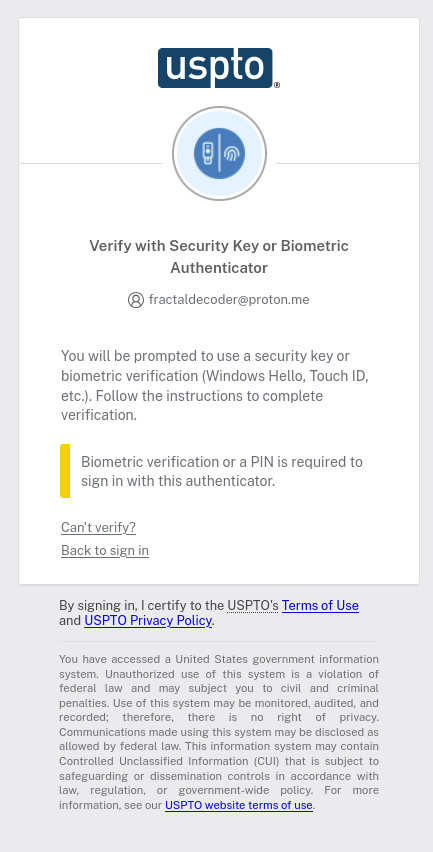
\includegraphics[width=0.6\textwidth]{Screenshot from 2026-03-14 21-25-17.png}
\caption{USPTO login portal on 2026-03-14, blocking access with
  mandatory security key / biometric verification.}
\end{figure}

\vspace{2em}
\noindent\rule{\textwidth}{0.4pt}

\vspace{1em}
\noindent\textit{Provisional Patent Application}\\
\textit{Inventor: Nick Spiker}\\
\textit{All rights reserved}

\end{document}